%20-25 min preso!
\documentclass[xcolor=table,aspectratio=169]{beamer}
\usepackage{beamerthemesplit}
\usepackage{wrapfig}
\usetheme{SPbGU}
\usepackage{pdfpages}
\usepackage{amsmath}
\usepackage{cmap}
\usepackage[T2A]{fontenc}
\usepackage[utf8]{inputenc}
\usepackage[english]{babel}
\usepackage{indentfirst}
\usepackage{amsmath}
\usepackage{tikz}
\usepackage{multirow}
\usepackage[noend]{algpseudocode}
\usepackage{algorithm}
\usepackage{algorithmicx}
\usepackage{fancyvrb}
\usepackage{hyperref} 
\usetikzlibrary{calc}
\usetikzlibrary{shapes, backgrounds}
\usetikzlibrary{arrows,automata}
\usetikzlibrary{positioning}
\usetikzlibrary{fit}
\usetikzlibrary{shapes.callouts}
\usetikzlibrary{shapes.misc}
\usepackage{xparse}
\usepackage{fontawesome}
\usepackage{minted}
\usepackage{color}


\usepackage{etoolbox,refcount}
\usepackage{multicol}

\usepackage{tabularx}
\newcolumntype{Y}{>{\raggedleft\arraybackslash}X}

\renewcommand{\thealgorithm}{}

\newtheorem{mytheorem}{Theorem}
\renewcommand{\thealgorithm}{}

\newcommand{\tikzmark}[1]{\tikz[overlay,remember picture] \node (#1) {};}
\def\Put(#1,#2)#3{\leavevmode\makebox(0,0){\put(#1,#2){#3}}}

\newcommand{\ltz}{$< 1$}

\tikzset{
    state/.style={
           rectangle,
           rounded corners,
           draw=black, very thick,
           minimum height=2em,
           inner sep=2pt,
           text centered,
           },
}

\tikzset{
    invisible/.style={opacity=0,text opacity=0},
    visible on/.style={alt=#1{}{invisible}},
    alt/.code args={<#1>#2#3}{%
      \alt<#1>{\pgfkeysalso{#2}}{\pgfkeysalso{#3}} % \pgfkeysalso doesn't change the path
    },
}

\tikzset{cross/.style={cross out, draw=black, minimum size=2*(#1-\pgflinewidth), inner sep=0pt, outer sep=0pt, ultra thick},
%default radius will be 1pt. 
cross/.default={1pt}}

\NewDocumentCommand{\mycallout}{r<> O{opacity=0.8,text opacity=1} m m m}{%
\tikz[remember picture, overlay]\node[align=center, fill=cyan!20, text width=#5cm,
#2,visible on=<#1>, rounded corners,
draw,rectangle callout,anchor=pointer,callout relative pointer={(290:0.5cm)}]
at (#3) {#4};
}

\NewDocumentCommand{\mycalloutR}{r<> O{opacity=0.8,text opacity=1} m m m}{%
\tikz[remember picture, overlay]\node[align=center, fill=cyan!20, text width=#5cm,
#2,visible on=<#1>, rounded corners,
draw,rectangle callout,anchor=pointer,callout relative pointer={(30:0.8cm)}]
at (#3) {#4};
}


%callout relative pointer={(230:0.5cm)}]
\setbeamertemplate{page number in head/foot}[appendixframenumber]
\newcounter{countitems}
\newcounter{nextitemizecount}
\newcommand{\setupcountitems}{%
  \stepcounter{nextitemizecount}%
  \setcounter{countitems}{0}%
  \preto\item{\stepcounter{countitems}}%
}
\makeatletter
\newcommand{\computecountitems}{%
  \edef\@currentlabel{\number\c@countitems}%
  \label{countitems@\number\numexpr\value{nextitemizecount}-1\relax}%
}
\newcommand{\nextitemizecount}{%
  \getrefnumber{countitems@\number\c@nextitemizecount}%
}
\newcommand{\previtemizecount}{%
  \getrefnumber{countitems@\number\numexpr\value{nextitemizecount}-1\relax}%
}
\makeatother    
\newenvironment{AutoMultiColItemize}{%
\ifnumcomp{\nextitemizecount}{>}{3}{\begin{multicols}{2}}{}%
\setupcountitems\begin{itemize}}%
{\end{itemize}%
\unskip\computecountitems\ifnumcomp{\previtemizecount}{>}{3}{\end{multicols}}{}}

\definecolor{links}{HTML}{2A1B81}
\hypersetup{colorlinks,linkcolor=,urlcolor=links}


\newcommand\colR{\cellcolor{red!20}}
\newcommand\colB{\cellcolor{blue!20}}
\newcommand\colG{\cellcolor{green!20}}

\beamertemplatenavigationsymbolsempty

\title[Brahma.FSharp: GPGPU + .NET]{Brahma.FSharp: Power of Functional Programming to Create Portable GPGPU-enabled .NET Applications} 
\institute[SPbSU]{
St. Petersburg State University
}

% То, что в квадратных скобках, отображается в левом нижнем углу.
\author[Semyon Grigorev]{Nikolai Ponomarev, Vladimir Kutuev, \underline{\textbf{Semyon Grigorev}}}

\date{October 7, 2025}


%Я предлагаю сначала в общем рассказать интересы и компетенции группы, 
%что научная группа сделала за 3 месяца, 
%потом потратить 1 страницу презентации на каждого из студентов (что сделал, почему важно для Yiming, какие планы). 
%В конце перейти к планам на год.

\begin{document}
{
\begin{frame}[fragile]
  \begin{table}
  \centering
  %
\includegraphics[height=1.5cm]{pictures/SPbGU_Logo.png}
  \begin{tabularx}{\linewidth}{XcX}
    
\includegraphics[height=1.4cm]{pictures/pact_2025_logo.png} \hfill
    & 
    & \hfill 
\includegraphics[height=1.6cm]{pictures/SPbGU_Logo.png}
  \end{tabularx}
  \end{table}
  \titlepage
\end{frame}
}

%In HPC or scintific computing we tend to create specific solution (eg supercomputer) to achieve maximal performance. In business applications we often want to increas performance using available hardware with minimal effort. Your laptop has intgrated GPU? Nice! We know that our software contains performance-critical part well-suited for GPUs. How can we easely offload this part of computatios to it?  

\begin{frame}[fragile]
  \frametitle{General-Purpose Computing on GPUs}
  \begin{itemize}
    \item Not only HPC and scientific computations
    \item Widely used in regular business applications
      \begin{itemize}
        \item Images and video processing
        \item AI/ML
        \item Financial analysis
        \item \ldots
      \end{itemize}
    \item Highest performance vs development simplification
      \begin{itemize}
        \item Native execution vs managed environments (JVM, .NET, etc)
        \item Low-level languages vs high-level ones
        \item \ldots
      \end{itemize}
    \item Functional languages for GPGPU 
      \begin{itemize}
        \item Type-safety, flexibility, advanced optimizations 
        \item Futhark, Lift, AnyDSL, \ldots
      \end{itemize}
    \end{itemize}
\end{frame}

\begin{frame}[fragile]
  \frametitle{.NET and F\#}
  \begin{itemize}
      \item .NET --- one of popular platforms for business applications development
      \item F\# --- functional-first programming language for .NET
      \begin{itemize}
        \item Statically strongly typed
        \begin{itemize}
          \item Type-safe development of generic kernels
        \end{itemize}
        \item F\# Code Quotations
        \begin{itemize}
          \item Compile-time metarogramming
          \item Runtime access to full-featured AST
          \item Statically typed
          \item Type-safe composition 
        \end{itemize}  
        \item F\# Mailbox Processor
        \begin{itemize}
          \item Integrated language-native primitive for message-passing-based asynchronous programming
        \end{itemize}
      \end{itemize}
    \end{itemize}
\end{frame}

\begin{frame}[fragile]
  \frametitle{F\# for GPGPU Programming: Design Decision Points}
  \begin{itemize}
    \item \textbf{Target technology}
    \begin{itemize}
      \item CUDA (\emph{e.g. Alea GPU}) --- mature stable infrastructure but Nvidia only
      \item OpenCL (\emph{e.g. FSCL}) --- wide range of devices and vendors
    \end{itemize}
    \item \textbf{Translator input}
    \begin{itemize}
      \item Bytecode (\emph{e.g. ILGPU}) --- one tool for all languages on the platform
      \item Source code (\emph{e.g. FSCL}) --- an ability to use language-specific features
    \end{itemize}
    \item \textbf{Control level}
    \begin{itemize}
      \item Fine-grained (\textit{e.g. ILGPU})
      \item black-box-like automatization (\textit{e.g. FSCL})
    \end{itemize}
    \item \textbf{Type safety}
    \begin{itemize} 
      \item None 
      \item Manual type annotations
      \item Automatic types inference and checking 
    \end{itemize}
    \item \textbf{Focus}
    \begin{itemize}
      \item Alea GPU: HPC, AI/ML, bindings for existing Cuda libs
      \item FSCL: automatic computation scheduling in heterogeneous systems
      \item \ldots
    \end{itemize}
  \end{itemize}
  
\end{frame}

%\begin{frame}[fragile]
%    \begin{center}
%    \begin{tabular}{|l|p{2.5cm}|l|l|p{3.5cm}|}
%      Tool          & Code access     & Target & Optimizations & Focus \\
%      \hline
%      \hline
%      Alea GPU      & Annotations     & Cuda C & & \\ 
%      FSCL          & Code quotations or annotations & OpenCL C & &  \\
%      ILGPU         & IL Annotations  & & \\
%      Brahma.FSharp & Code quotations & OpenCL C & \faCheck & Simple development \\
%    \end{tabular}
%  \end{center}
%\end{frame}

\begin{frame}[fragile]
  \frametitle{Brahma.FSharp}
  is a \textbf{F\# quotation to OpenCL translator} and respective \textbf{runtime} to utilize GPGPUs in F\# applications
  \begin{itemize}
    \item \textbf{Target technology}: OpenCL
    \item \textbf{Translator input}: source code (using quotations)
    \begin{itemize}
      \item Not only primitive types, but also discriminated unions, structs, records
      \item Pattern matching, mutable and immutable bindings, nested bindings
    \end{itemize}
    \item \textbf{Control level}: fine-grained memory management and kernels compilation process 
    \item \textbf{Type safety}: automatic
    \begin{itemize}
      \item Ten lines of types' manipulation magic that carefully build type for compiled kernel\footnote{\ldots and brakes some F\# compiler optimizations}
    \end{itemize}
    \item \textbf{Focus}: safety, static checks, development simplification
    \item Mailbox Processor wrapper for command queue
    \begin{itemize}
      \item Native way to integrate communication with GPGPUs into asynchronous pipelines
    \end{itemize}  
  \end{itemize}
\end{frame}

\begin{frame}[fragile]
  \frametitle{Research Questions}
  \begin{itemize}
    \item Can we create code portable across different devices and vendors?
    \item Can we create generic type-safe kernels?
    \item Can we utilize well-established optimizations if necessary?
    \item Does Mailbox Processor allows one to create asynchronous workflows that utilize heterogeneous devices?
\end{itemize}
\end{frame}


\begin{frame}[fragile]
  \frametitle{An Example of Generic Matrix Multiplication Kernel}
  \vspace{-0.6cm}
  \tikzmark{codeStart}{ }
  \begin{minted}[linenos]{fsharp}
  let mXmKernel (opAdd: Quotations.Expr<'a -> 'b -> 'a>) 
                (opMult: Quotations.Expr<'e -> 'f -> 'b>) 
                (zero: Quotations.Expr<'a>) ... (* other parameters *)  =
        ... // Supplementary code
        let kernel = <@ fun 2dRange m1 m2 res ->  // Quoted code
          ... 
          let acc = %zero // Embedded identity value
          let lBuf = localArray lws // captured from context
          ... 
          acc <- (%opAdd) acc ((%opMult) x y) // Embedded operations
          ... @>
        ... // Supplementary code
  
  let intArithmeticKernel = mXmKernel <@ (+) @> <@ ( * ) @> <@ 0 @>
  let intMinPlusKernel = mXmKernel <@ (min) @> <@ (+) @> <@ Int.MaxValue @>
    \end{minted}
    \onslide<2>{
    \tikz[overlay,remember picture]{\draw[draw=blue,thick,double,fill opacity=0.2] ($ (codeStart) + (3.2,-0.1)$) rectangle ($ (codeStart) + (11.4,-1.6)$);}
    }
    \onslide<3>{
    \tikz[overlay,remember picture]{\draw[draw=blue,thick,double,fill opacity=0.2] ($ (codeStart) + (1.5,-2.1)$) rectangle ($ (codeStart) + (13.6,-5.4)$);}
    }
    \onslide<4>{
    \tikz[overlay,remember picture]{\draw[draw=blue,thick,double,fill opacity=0.2] ($ (codeStart) + (4.7,-2.1)$) rectangle ($ (codeStart) + (9.1,-2.5)$);}
    }
    \onslide<5>{
    \tikz[overlay,remember picture]{\draw[draw=blue,thick,double,fill opacity=0.2] ($ (codeStart) + (1.9,-3.0)$) rectangle ($ (codeStart) + (10.5,-3.5)$);}
    \tikz[overlay,remember picture]{\draw[draw=blue!30,thick,double,fill opacity=0.2] ($ (codeStart) + (3.2,-1.1)$) rectangle ($ (codeStart) + (8.6,-1.6)$);}
    }
    \onslide<6>{
    \tikz[overlay,remember picture]{\draw[draw=blue,thick,double,fill opacity=0.2] ($ (codeStart) + (1.9,-3.5)$) rectangle ($ (codeStart) + (12.1,-4.0)$);}
    }
    \onslide<7>{
    \tikz[overlay,remember picture]{\draw[draw=blue!30,thick,double,fill opacity=0.2] ($ (codeStart) + (3.2,-0.1)$) rectangle ($ (codeStart) + (11.4,-1.1)$);}
    \tikz[overlay,remember picture]{\draw[draw=blue!30,thick,double,fill opacity=0.2] ($ (codeStart) + (1.9,-4.45)$) rectangle ($ (codeStart) + (13.8,-4.95)$);}
    \tikz[overlay,remember picture]{\draw[draw=blue,thick,double,fill opacity=0.2] ($ (codeStart) + (0.2,-6.35)$) rectangle ($ (codeStart) + (15.0,-7.4)$);}
    }

\end{frame}


\begin{frame}[fragile]
  \frametitle{Matrix Multiplication Evaluation: Environment}
  \begin{itemize}
    \item Optimizations
    \begin{itemize}
      \item Tiling in local and private memory\footnote{Inspired by ``\href{https://cnugteren.github.io/tutorial/pages/page1.html}{Tutorial: OpenCL SGEMM tuning for Kepler}'' by Cedric Nugteren} 
      \item Square matrices and square tiles
    \end{itemize}
    \item Hardware
    \begin{itemize}
      \item \textbf{Lenovo}: Intel Core i7-8550U CPU, NVIDIA GeForce MX150 and Intel UHD Graphics 620 GPUs
      \item \textbf{Zen}: Intel Core i5-1340P CPU, Intel Iris Xe Graphics G7 80EUs GPU
      \item \textbf{MILK-V}: SpacemiT M1 CPU, IMG BXE-2-32 GPU
    \end{itemize} 
    \item Software
    \begin{itemize}
      \item \textbf{CLBlast}: optimized OpenCL-based BLAS implementation tuned for low-power mobile GPUs
      \item \textbf{OpenBLAS}: optimized CPU-based BLAS implementation
    \end{itemize}
    \item \textbf{PoCL} to execute OpenCL-based solutions on CPUs
\end{itemize}

\end{frame}

\begin{frame}[t]
  \frametitle{Matrix Multiplication Performance: \textbf{Lenovo} and \textbf{Zen}}
  \tikzmark{figStart1}
  \begin{center}
    \vfill
    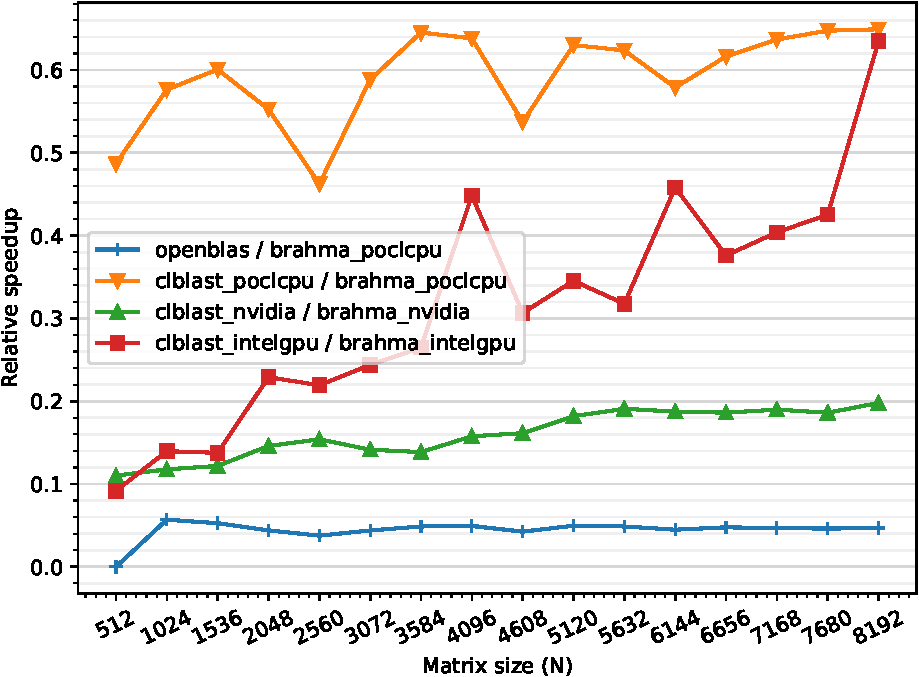
\includegraphics[width=0.49\textwidth]{../data/Lenovo-T480_rel_crop.pdf}
    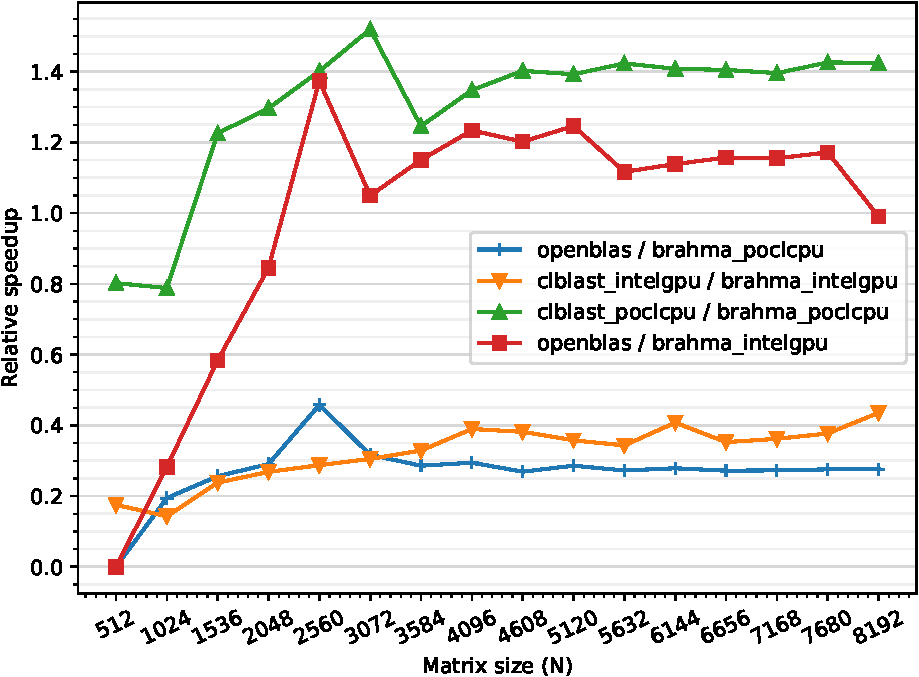
\includegraphics[width=0.49\textwidth]{../data/zenbook_iris_rel_crop.pdf}
  \end{center}
  \onslide<5>{
    \tikz[overlay,remember picture]{\draw[draw=blue,thick,double,fill opacity=0.2] ($ (figStart1) + (0.8,-3.05)$) rectangle ($ (figStart1) + (4.4,-3.4)$);}
    }
  \onslide<4>{
    \tikz[overlay,remember picture]{\draw[draw=blue,thick,double,fill opacity=0.2] ($ (figStart1) + (0.8,-2.8)$) rectangle ($ (figStart1) + (4.4,-3.1)$);}
    \tikz[overlay,remember picture]{\draw[draw=blue,thick,double,fill opacity=0.2] ($ (figStart1) + (11.5,-2.55)$) rectangle ($ (figStart1) + (15.1,-2.85)$);}
    }
  \onslide<3>{
    \tikz[overlay,remember picture]{\draw[draw=blue,thick,double,fill opacity=0.2] ($ (figStart1) + (0.8,-2.55)$) rectangle ($ (figStart1) + (4.4,-2.85)$);}
    \tikz[overlay,remember picture]{\draw[draw=blue,thick,double,fill opacity=0.2] ($ (figStart1) + (11.5,-2.8)$) rectangle ($ (figStart1) + (15.1,-3.1)$);}
    }
\onslide<2>{
    \tikz[overlay,remember picture]{\draw[draw=blue,thick,double,fill opacity=0.2] ($ (figStart1) + (0.8,-2.3)$) rectangle ($ (figStart1) + (4.4,-2.6)$);}
    \tikz[overlay,remember picture]{\draw[draw=blue,thick,double,fill opacity=0.2] ($ (figStart1) + (11.5,-2.3)$) rectangle ($ (figStart1) + (15.1,-2.6)$);}
    }    


\end{frame}

%\begin{frame}[t]
%  \frametitle{Matrix Multiplication Performance: \textbf{Lenovo}}
%  \begin{center}
%    \vfill
%    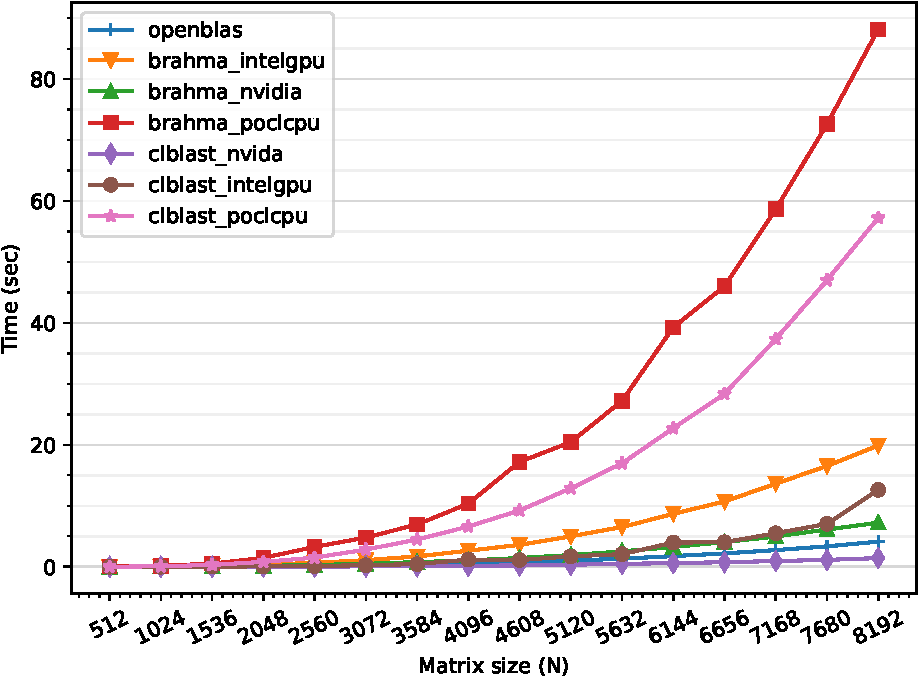
\includegraphics[width=0.49\textwidth]{../data/Lenovo-T480_crop.pdf}
%    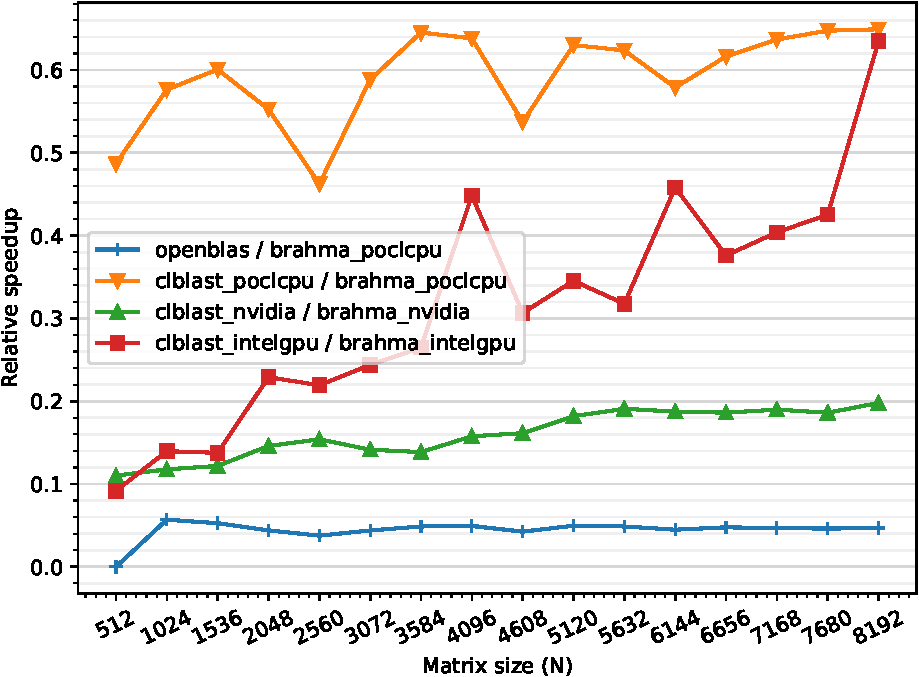
\includegraphics[width=0.49\textwidth]{../data/Lenovo-T480_rel_crop.pdf}
%  \end{center}
%\end{frame}

%\begin{frame}[t]
%  \frametitle{Matrix Multiplication Performance: \textbf{Zen}}
%  \begin{center}
%    \vfill  
%    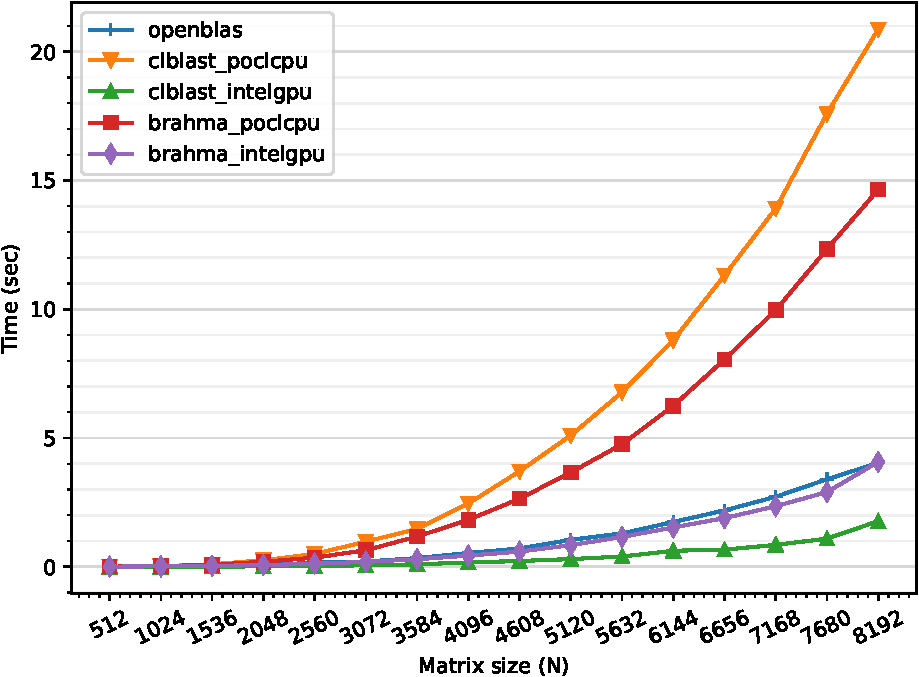
\includegraphics[width=0.49\textwidth]{../data/zenbook_iris_crop.pdf}
%    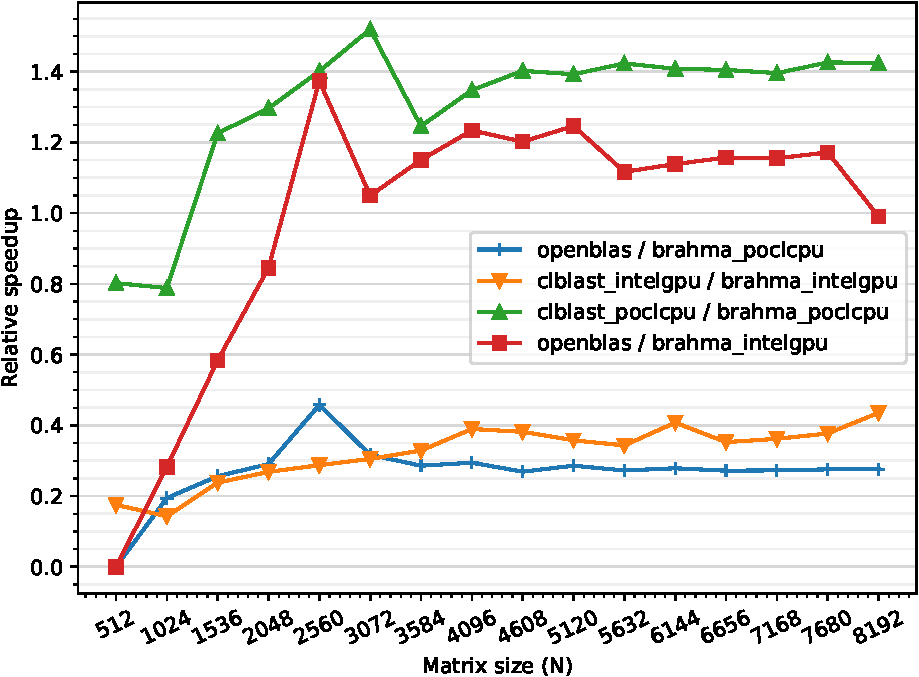
\includegraphics[width=0.49\textwidth]{../data/zenbook_iris_rel_crop.pdf}
%  \end{center}
%\end{frame}

\begin{frame}[t]
  \frametitle{Matrix Multiplication Performance: \textbf{MILK-V}}
  \tikzmark{figStart2}
  \begin{center}
    \vfill
    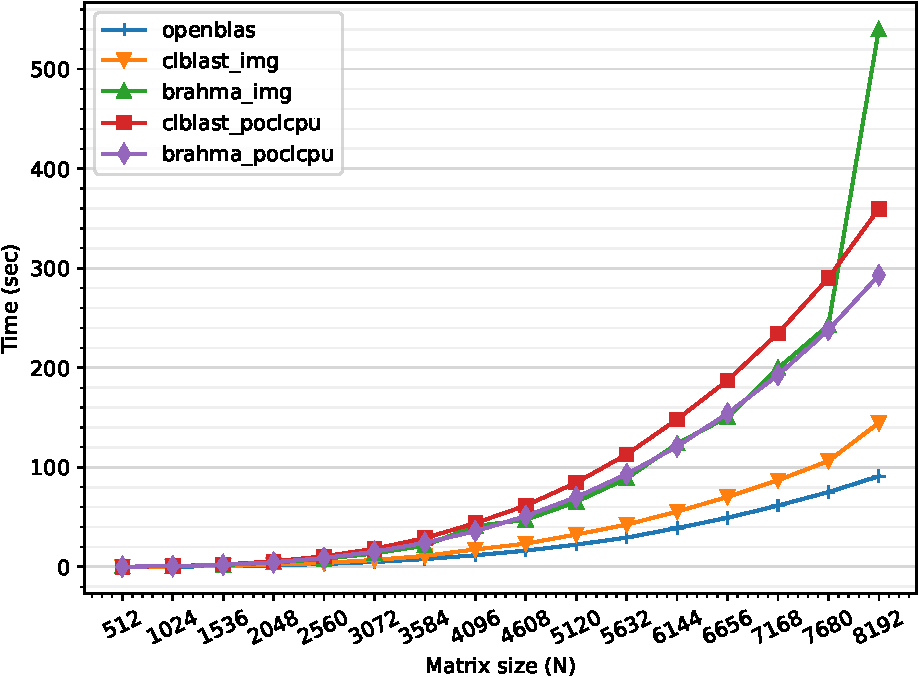
\includegraphics[width=0.49\textwidth]{../data/MILK-V_crop.pdf}
    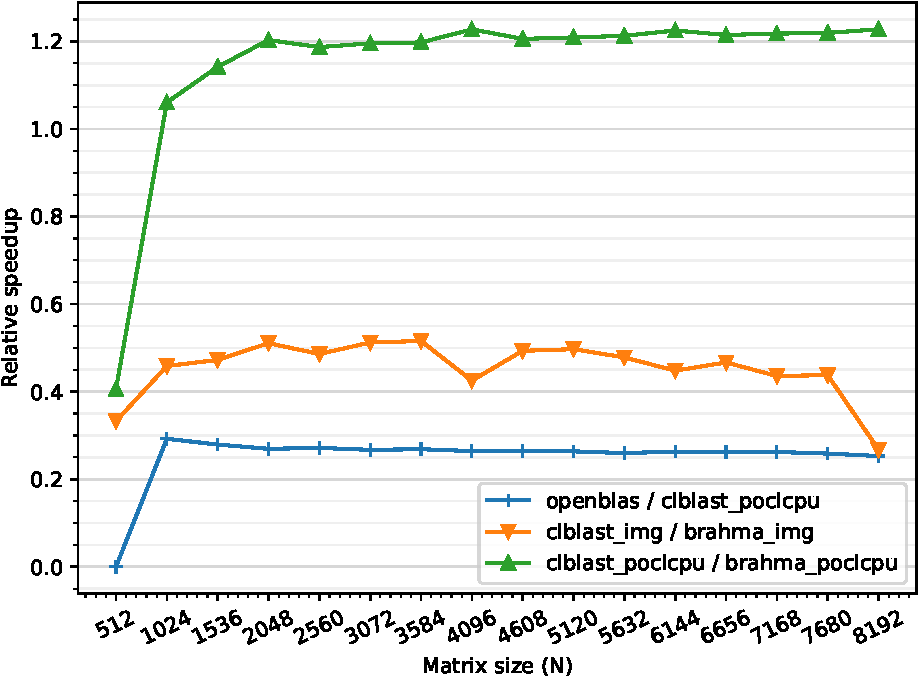
\includegraphics[width=0.49\textwidth]{../data/MILK-V_rel_crop.pdf}
  \end{center}
  \onslide<2>{
    \tikz[overlay,remember picture]{\draw[draw=blue,thick,double,fill opacity=0.2] ($ (figStart1) + (0.8,-0.5)$) rectangle ($ (figStart1) + (2.85,-1.1)$);}
    }
\end{frame}

\begin{frame}[fragile]
  \frametitle{Image Processing Using Mailbox Processor\footnote{Basic version}}
\tikzmark{codeStart2}
\begin{minted}[linenos]{fsharp}
let imgProcessor filter (imgSaver: MailboxProcessor<_>) =
    MailboxProcessor.Start(fun inbox ->
        let rec loop ... = async { // Async message processing loop
            let! msg = inbox.Receive() // Load message
            match msg with
            | EOS ch -> // Handle end of stream
                imgSaver.PostAndReply EOS
                ch.Reply()
            | Img img -> // Handle image
                let filtered = filter img // Convolution
                imgSaver.Post (Img filtered)
                return! loop ... }// Got to next message
        loop ...)
  \end{minted}
  \onslide<2>{
    \tikz[overlay,remember picture]{\draw[draw=blue,thick,double,fill opacity=0.2] ($ (codeStart2) + (1.2,-1.1)$) rectangle ($ (codeStart2) + (13.85,-5.9)$);}
    }
  \onslide<3>{
    \tikz[overlay,remember picture]{\draw[draw=blue,thick,double,fill opacity=0.2] ($ (codeStart2) + (2.2,-1.55)$) rectangle ($ (codeStart2) + (11.65,-2.05)$);}
    }
  \onslide<4>{
    \tikz[overlay,remember picture]{\draw[draw=blue,thick,double,fill opacity=0.2] ($ (codeStart2) + (2.2,-2.5)$) rectangle ($ (codeStart2) + (11.65,-3.95)$);}
    }
    \onslide<5>{
    %\tikz[overlay,remember picture]{\draw[draw=blue,thick,double,fill opacity=0.2] ($ (figStart1) + (2.2,-3.5)$) rectangle ($ (figStart1) + (11.65,-4.95)$);}
    \tikz[overlay,remember picture]{\draw[draw=blue,thick,double,fill opacity=0.2] ($ (codeStart2) + (2.2,-3.95)$) rectangle ($ (codeStart2) + (11.65,-5.9)$);}
    }
    \onslide<6>{
      \tikz[overlay,remember picture]{\draw[draw=blue!30,thick,double,fill opacity=0.2] ($ (codeStart2) + (2.2,-3.95)$) rectangle ($ (codeStart2) + (11.65,-5.9)$);}
    \tikz[overlay,remember picture]{\draw[draw=blue,thick,double,fill opacity=0.2] ($ (codeStart2) + (2.2,-4.9)$) rectangle ($ (codeStart2) + (11.65,-5.4)$);}
    }
    \onslide<7>{
      \tikz[overlay,remember picture]{\draw[draw=blue!30,thick,double,fill opacity=0.2] ($ (codeStart2) + (2.2,-3.95)$) rectangle ($ (codeStart2) + (11.65,-5.9)$);}
    \tikz[overlay,remember picture]{\draw[draw=blue,thick,double,fill opacity=0.2] ($ (codeStart2) + (2.2,-5.4)$) rectangle ($ (codeStart2) + (11.65,-5.9)$);}
    }  
\end{frame}


\begin{frame}[fragile]
  \frametitle{Evaluaiton of Image Processing}

\begin{itemize}
  \item Environment
  \begin{itemize}
    \item \textbf{Lenovo}: Intel Core i7-8550U CPU, NVIDIA GeForce MX150 and Intel UHD Graphics 620 GPUs
    \item Stream processing: 420 images (1Gb of data), load--process--store
    \item $5 \times 5$ kernels sequence: 3 Gaussian blur, 1 edge detection
  \end{itemize}
  \item Results
  \begin{itemize}
    \item 64 seconds on Nvidia GPU
    \item 97 seconds on Intel GPU
    \item 40 seconds using Intel and Nvidia simultaneously: \textbf{30\% speedup} 
  \end{itemize}
\end{itemize}  
\end{frame}


\begin{frame}[t]
  \frametitle{Conclusion}
  \begin{itemize}
    \item Brahma.FSharp allows one to create portable solutions
    \begin{itemize}
      \item We want to create homogeneous code\footnote{Even .NET-only, without wrappers for native libraries} to simplify development and portability process\footnote{Write once, run everywhere. In some cases.} 
    \end{itemize}
    \item Brahma.FSharp allows one to create highly-parameterizable type-safe kernels 
    \begin{itemize}
      \item Code support simplification: single highly-optimized  and type-safe kernel\footnote{But without type-specific optimizations}
    \end{itemize}
    \item Brahma.FSharp allows one to utilize well-established optimizations 
    \begin{itemize}
      \item Including manipulations with local and private memory
    \end{itemize}
    \item Mailbox Processor allows one 
    \begin{itemize}
      \item To create asynchronous workflows that utilize heterogeneous environment in F\#-native way 
      \item To utilize heterogeneous devices to increase performance 
    \end{itemize}
    
    \vfill
    \item We should reduce runtime overhead
    \item In case of matrix multiplication, there is a room for kernels tuning
  \end{itemize}
\end{frame}

\begin{frame}[fragile]
  \frametitle{Useful Links}
  \begin{minipage}{0.70\textwidth}
  \begin{itemize}
    \item Brahma.FSharp sources: \url{https://github.com/YaccConstructor/Brahma.FSharp}
    \item Environment for evaluation and examples: \url{https://github.com/gsvgit/ImageProcessing}
  \end{itemize}
\end{minipage}
\begin{minipage}[t]{0.29\textwidth}
  \begin{center}
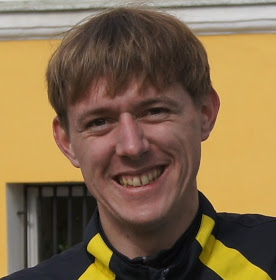
\includegraphics[width=0.8\textwidth]{pictures/SemyonGrigorev.jpg}
  \end{center}
  {\scriptsize
\begin{itemize}    
  \item Email: s.v.grigoriev@mail.spbu.ru
  \item GitHub: \href{https://github.com/gsvgit}{gsvgit}
  \item Google Scholar: \href{https://scholar.google.com/citations?hl=ru&user=kP4dqUAAAAAJ&view_op=list_works&sortby=pubdate}{Semyon Grigorev}
  \item DBLP: \href{https://dblp.org/pid/181/9903.html}{Semyon V. Grigorev}
\end{itemize}
  }
\end{minipage}
\end{frame}

\end{document}
